\documentclass[12pt,a4paper,oneside]{report}

% --- CẤU HÌNH NGÔN NGỮ VÀ PHÔNG CHỮ ĐA TƯƠNG THÍCH (pdflatex, xelatex, lualatex) ---
\usepackage{iftex}
\ifPDFTeX
  \usepackage[utf8]{inputenc}
  \usepackage[T5]{fontenc}
  \usepackage[vietnamese]{babel}
  \renewcommand{\rmdefault}{ptm}
  \usepackage{newunicodechar}
  \newunicodechar{–}{--}
  \newunicodechar{—}{---}
  \newunicodechar{“}{``}
  \newunicodechar{”}{''}
  \newunicodechar{…}{\dots}
  \newunicodechar{×}{\ensuremath{\times}}
\else
  \usepackage{fontspec}
  \usepackage[vietnamese]{babel}
  \setmainfont{Times New Roman}
\fi

% --- ĐỊNH DẠNG TRANG VÀ LỀ THEO CHUẨN ĐỒ ÁN / LUẬN VĂN ---
\usepackage[a4paper,top=25mm,bottom=25mm,left=30mm,right=20mm]{geometry}
\usepackage{setspace}
\onehalfspacing
\setlength{\parindent}{1cm}
\setlength{\parskip}{4pt}

% --- CÁC GÓI BỔ TRỢ HÌNH ẢNH, BẢNG BIỂU, MÀU SẮC ---
\usepackage{graphicx}
\graphicspath{{images/}}
\usepackage{booktabs}
\usepackage{longtable}
\usepackage{tabularx}
\usepackage{array}
\usepackage{makecell}
\usepackage{multirow}
\usepackage[table]{xcolor}
\usepackage{titlesec}
\usepackage{enumitem}
\usepackage{fancyhdr}
\usepackage{caption}
\usepackage{tikz}
\usetikzlibrary{calc}
\usepackage[unicode,colorlinks=true,linkcolor=black,citecolor=blue,urlcolor=blue]{hyperref}

% --- ĐỊNH NGHĨA MÀU SẮC GIAO DIỆN VÀ MÀU KHUNG BÌA TRƯỜNG CTUT ---
\definecolor{ctutBlue}{HTML}{004386}
\definecolor{etvSurface}{HTML}{FEF3C7}
\definecolor{etvNav}{HTML}{1F3B54}
\definecolor{etvSelected}{HTML}{A1C4E9}
\definecolor{etvPrimary}{HTML}{0047AB}
\definecolor{etvInk}{HTML}{0F172A}
\definecolor{etvMuted}{HTML}{475569}
\definecolor{etvSuccess}{HTML}{16A34A}
\definecolor{etvWarning}{HTML}{D97706}
\definecolor{etvDanger}{HTML}{DC2626}

% Lệnh tạo ô mẫu màu giao diện trực quan
\newcommand{\colorsample}[1]{\fcolorbox{gray!60}{#1}{\rule{0pt}{2mm}\rule{10mm}{0pt}}}

% --- ĐỊNH DẠNG TIÊU ĐỀ MỤC ---
\titleformat{\chapter}[hang]
  {\normalfont\bfseries\Large\centering}
  {CHƯƠNG \thechapter:}{0.5em}{\MakeUppercase}
\titlespacing*{\chapter}{0pt}{10pt}{20pt}

\titleformat{\section}
  {\normalfont\bfseries\large}
  {\thesection.}{0.5em}{}
\titlespacing*{\section}{0pt}{12pt}{6pt}

\titleformat{\subsection}
  {\normalfont\bfseries\normalsize}
  {\thesubsection.}{0.5em}{}
\titlespacing*{\subsection}{0pt}{10pt}{4pt}

\titleformat{\subsubsection}
  {\normalfont\bfseries\itshape\normalsize}
  {\thesubsubsection.}{0.5em}{}
\titlespacing*{\subsubsection}{0pt}{8pt}{4pt}

% --- ĐỊNH DẠNG TÊN DANH MỤC VÀ CHÚ THÍCH ---
\renewcommand{\contentsname}{MỤC LỤC}
\renewcommand{\listfigurename}{DANH MỤC HÌNH ẢNH}
\renewcommand{\listtablename}{DANH MỤC BẢNG BIỂU}
\captionsetup[table]{name=Bảng,labelsep=colon,justification=centering}
\captionsetup[figure]{name=Hình,labelsep=colon,justification=centering}

% --- CẤU HÌNH DANH SÁCH ---
\setlist[itemize]{topsep=2pt,partopsep=0pt,itemsep=2pt,parsep=2pt,leftmargin=1.5cm}
\setlist[enumerate]{topsep=2pt,partopsep=0pt,itemsep=2pt,parsep=2pt,leftmargin=1.5cm}

\begin{document}

% ==============================================================================
% TRANG BÌA CHÍNH (CÓ KHUNG VIỀN ĐỒ ÁN - CHỈ CÓ TÊN SINH VIÊN, KHÔNG CÓ GVHD/MSSV)
% ==============================================================================
\begin{titlepage}
\begin{tikzpicture}[remember picture, overlay]
  % Khung đôi trang bìa theo chuẩn màu xanh CTUT #004386
  \draw[line width=2.5pt, color=ctutBlue]
    ($(current page.north west) + (25mm,-20mm)$)
    rectangle
    ($(current page.south east) + (-15mm,20mm)$);
  \draw[line width=0.8pt, color=ctutBlue]
    ($(current page.north west) + (26.5mm,-21.5mm)$)
    rectangle
    ($(current page.south east) + (-16.5mm,21.5mm)$);
\end{tikzpicture}

\begin{center}
  \vspace*{-0.2cm}
  {\fontsize{13}{16}\selectfont TRƯỜNG ĐẠI HỌC KỸ THUẬT -- CÔNG NGHỆ CẦN THƠ}\\[4pt]
  {\fontsize{13}{16}\selectfont \textbf{KHOA CÔNG NGHỆ THÔNG TIN}}\\[0.8cm]

  
\includegraphics[width=4.2cm]{image1.png}\\[1.2cm]

  {\fontsize{15}{19}\selectfont \textbf{BÁO CÁO ĐỒ ÁN HỌC PHẦN}}\\[8pt]
  {\fontsize{15}{19}\selectfont \textbf{THIẾT KẾ GIAO DIỆN NGƯỜI DÙNG ĐỒ HỌA}}\\[1.5cm]

  {\fontsize{15}{20}\selectfont \textbf{THIẾT KẾ UI/UX CHO NỀN TẢNG ĐÁNH GIÁ CODE\\[6pt]VÀ TRỢ GIẢNG ẢO}}\\[2.5cm]

  {\fontsize{13}{17}\selectfont \textbf{NGUYỄN MINH THÙY}}\\[8pt]
  {\fontsize{13}{17}\selectfont \textbf{NGÔ THU VÂN}}

  \vfill

  {\fontsize{13}{16}\selectfont \textbf{Cần Thơ, năm 2026}}\\[0.2cm]
\end{center}
\end{titlepage}

% ==============================================================================
% TRANG BÌA PHỤ (CÓ KHUNG VIỀN ĐỒ ÁN, ĐẦY ĐỦ CÁN BỘ HƯỚNG DẪN VÀ SINH VIÊN + MSSV)
% ==============================================================================
\begin{titlepage}
\begin{tikzpicture}[remember picture, overlay]
  % Khung đôi trang bìa theo chuẩn màu xanh CTUT #004386
  \draw[line width=2.5pt, color=ctutBlue]
    ($(current page.north west) + (25mm,-20mm)$)
    rectangle
    ($(current page.south east) + (-15mm,20mm)$);
  \draw[line width=0.8pt, color=ctutBlue]
    ($(current page.north west) + (26.5mm,-21.5mm)$)
    rectangle
    ($(current page.south east) + (-16.5mm,21.5mm)$);
\end{tikzpicture}

\begin{center}
  \vspace*{-0.2cm}
  {\fontsize{13}{16}\selectfont TRƯỜNG ĐẠI HỌC KỸ THUẬT -- CÔNG NGHỆ CẦN THƠ}\\[4pt]
  {\fontsize{13}{16}\selectfont \textbf{KHOA CÔNG NGHỆ THÔNG TIN}}\\[0.8cm]

  
\includegraphics[width=4.2cm]{image1.png}\\[1.2cm]

  {\fontsize{15}{19}\selectfont \textbf{BÁO CÁO ĐỒ ÁN HỌC PHẦN}}\\[8pt]
  {\fontsize{15}{19}\selectfont \textbf{THIẾT KẾ GIAO DIỆN NGƯỜI DÙNG ĐỒ HỌA}}\\[1.2cm]

  {\fontsize{15}{20}\selectfont \textbf{THIẾT KẾ UI/UX CHO NỀN TẢNG ĐÁNH GIÁ CODE\\[6pt]VÀ TRỢ GIẢNG ẢO}}
\end{center}

\vfill

\noindent
\hspace*{0.5cm}%
\begin{tabular}{@{}p{8.0cm}p{7.0cm}@{}}
  {\fontsize{13}{17}\selectfont Cán bộ hướng dẫn:} & {\fontsize{13}{17}\selectfont Sinh viên thực hiện:} \\[6pt]
  {\fontsize{13}{17}\selectfont \textbf{Th.S ĐẶNG THỊ DUNG}} & {\fontsize{13}{17}\selectfont \textbf{NGUYỄN MINH THÙY}} \\[4pt]
  & {\fontsize{13}{17}\selectfont \textbf{MSSV: CNTT2311090}} \\[6pt]
  & {\fontsize{13}{17}\selectfont \textbf{NGÔ THU VÂN}} \\[4pt]
  & {\fontsize{13}{17}\selectfont \textbf{MSSV: CNTT2311044}} \\
\end{tabular}

\vfill

\begin{center}
  {\fontsize{13}{16}\selectfont \textbf{Cần Thơ, năm 2026}}\\[0.2cm]
\end{center}
\vspace*{-0.5cm}
\end{titlepage}

% ==============================================================================
% CÁC TRANG ĐẦU TIÊN (ĐÁNH SỐ LA MÃ)
% ==============================================================================
\pagenumbering{roman}
\setcounter{page}{1}

% --- NHẬN XÉT CỦA GIẢNG VIÊN HƯỚNG DẪN ---
\chapter*{NHẬN XÉT CỦA GIẢNG VIÊN HƯỚNG DẪN}
\addcontentsline{toc}{chapter}{Nhận xét của giảng viên hướng dẫn}

\noindent\makebox[\linewidth]{\dotfill}\\[0.7cm]
\noindent\makebox[\linewidth]{\dotfill}\\[0.7cm]
\noindent\makebox[\linewidth]{\dotfill}\\[0.7cm]
\noindent\makebox[\linewidth]{\dotfill}\\[0.7cm]
\noindent\makebox[\linewidth]{\dotfill}\\[0.7cm]
\noindent\makebox[\linewidth]{\dotfill}\\[0.7cm]
\noindent\makebox[\linewidth]{\dotfill}\\[0.7cm]
\noindent\makebox[\linewidth]{\dotfill}\\[0.7cm]
\noindent\makebox[\linewidth]{\dotfill}\\[0.7cm]
\noindent\makebox[\linewidth]{\dotfill}

\vspace{1.5cm}

\begin{flushright}
  \textit{Cần Thơ, ngày \dots\dots\ tháng \dots\dots\ năm 2026}\\[4pt]
  \textbf{Giảng viên hướng dẫn}\\[4pt]
  \textit{(Ký và ghi rõ họ tên)}\\[2.5cm]
  \textbf{ThS. Đặng Thị Dung}
\end{flushright}

\newpage

% --- LỜI CAM ĐOAN ---
\chapter*{LỜI CAM ĐOAN}
\addcontentsline{toc}{chapter}{Lời cam đoan}

Chúng em xin được cam đoan đề tài \textbf{``Thiết kế UI/UX cho Nền tảng Đánh giá Code và Trợ giảng Ảo''} được tiến hành công khai, là công trình nghiên cứu dựa trên sự cố gắng, nỗ lực của chúng em, cũng như là kết quả của quá trình học tập, nghiên cứu và thực hiện nghiêm túc của chúng em, dưới sự hướng dẫn tận tình của ThS. Đặng Thị Dung.

Các số liệu và kết quả nghiên cứu của đề tài là trung thực, không sao chép hoặc sử dụng kết quả của đề tài nghiên cứu nào tương tự. Tất cả những sự giúp đỡ cho việc xây dựng cơ sở lý thuyết đều được trích dẫn đầy đủ và ghi nguồn gốc rõ ràng và được phép công bố.

Chúng em xin chịu hoàn toàn trách nhiệm nếu có sự không trung thực trong thông tin sử dụng trong công trình nghiên cứu này.

\vspace{1.5cm}

\begin{flushright}
  \textit{Cần Thơ, ngày \dots\dots\ tháng \dots\dots\ năm 2026}\\[4pt]
  \textbf{Sinh viên thực hiện}\\[4pt]
  \textit{(Ký và ghi rõ họ tên)}\\[2.5cm]
\end{flushright}

\begin{center}
\begin{tabular}{p{0.45\textwidth}p{0.45\textwidth}}
  \centering \textbf{Nguyễn Minh Thùy} & \centering \textbf{Ngô Thu Vân}
\end{tabular}
\end{center}

\newpage

% --- LỜI CẢM ƠN ---
\chapter*{LỜI CẢM ƠN}
\addcontentsline{toc}{chapter}{Lời cảm ơn}

Trong khoảng thời gian làm báo cáo học phần, chúng em đã nhận được nhiều sự giúp đỡ, đóng góp ý kiến và sự dẫn dắt chỉ bảo nhiệt tình của thầy cô, gia đình và bạn bè.

Đặc biệt chúng em xin gửi lời cảm ơn chân thành đến giáo viên hướng dẫn -- ThS. Đặng Thị Dung, giảng viên Trường Đại học Kỹ thuật -- Công nghệ Cần Thơ, người đã tận tình hướng dẫn, chỉ bảo em trong suốt quá trình làm đồ án.

Chúng em cũng xin gửi cảm ơn chân thành nhất tới các thầy cô giáo trong trường Đại học Kỹ thuật -- Công nghệ Cần Thơ nói chung, các thầy cô trong Bộ môn Công nghệ thông tin nói riêng đã dạy dỗ cho chúng em kiến thức về các môn đại cương cũng như các môn chuyên ngành, giúp chúng em có được cơ sở lý thuyết vững vàng và tạo điều kiện giúp đỡ chúng em trong suốt quá trình chúng em tham gia học tập.

Cuối cùng, chúng em xin chân thành cảm ơn gia đình và bạn bè, những người luôn ở bên cạnh đã luôn tạo điều kiện, quan tâm, giúp đỡ, động viên chúng em trong suốt quá trình học tập và hoàn thành đồ án.

Với điều kiện về thời gian cũng như lượng kiến thức về đề tài rất rộng mà kinh nghiệm còn hạn chế của chúng em, báo cáo học phần này không thể tránh được những thiếu sót. Chúng em rất mong nhận được sự chỉ bảo, đóng góp ý kiến của các thầy cô để chúng em có điều kiện bổ sung, nâng cao ý thức của mình, phục vụ tốt hơn công tác thực tế sau này.

Chúng em xin chân thành cảm ơn!

\newpage

% --- TÓM TẮT ---
\chapter*{TÓM TẮT}
\addcontentsline{toc}{chapter}{Tóm tắt}

Đề tài \textbf{``Thiết kế UI/UX cho Nền tảng Đánh giá Code và Trợ giảng Ảo''} được thực hiện nhằm nghiên cứu, phân tích và thiết kế giao diện người dùng (UI), đồng thời xây dựng trải nghiệm người dùng (UX) cho một nền tảng hỗ trợ hoạt động dạy và học lập trình.

Trong phạm vi đề tài, nhóm tập trung xác định các đối tượng sử dụng và nhu cầu tương ứng, xây dựng chân dung người dùng (User Persona), sơ đồ tổng quan hệ thống, sơ đồ phân cấp chức năng (Sitemap) và các luồng tương tác chính (User Flow). Hệ thống hướng đến năm nhóm người dùng gồm: Sinh viên, Giáo viên, Giáo vụ, Quản trị viên và Quản trị viên hệ thống. Các chức năng được nghiên cứu bao gồm quản lý bài tập, tổ chức lớp học, viết và nộp mã nguồn, theo dõi kết quả chấm bài, hỗ trợ học tập bằng AI và quản trị hệ thống.

Trên cơ sở phân tích yêu cầu, nhóm tiến hành thiết kế giao diện trên nền tảng Figma, chú trọng tính nhất quán, khả năng điều hướng, tính trực quan và khả năng thích ứng trên nhiều kích thước thiết bị. Các luồng tương tác được xây dựng nhằm mô phỏng quá trình sử dụng hệ thống của từng nhóm người dùng.

Kết quả của đề tài là bộ thiết kế giao diện UI/UX và prototype trên Figma, làm cơ sở tham khảo cho quá trình đánh giá trải nghiệm người dùng và phát triển hệ thống trong tương lai. Đề tài tập trung vào khía cạnh phân tích, thiết kế giao diện và mô phỏng tương tác, không đi sâu vào triển khai backend, cơ sở dữ liệu hoặc vận hành hệ thống thực tế.

\newpage

% --- MỤC LỤC ---
\tableofcontents
\newpage

% --- DANH MỤC CÁC TỪ VIẾT TẮT VÀ THUẬT NGỮ ---
\chapter*{DANH MỤC CÁC TỪ VIẾT TẮT VÀ THUẬT NGỮ}
\addcontentsline{toc}{chapter}{Danh mục các từ viết tắt và thuật ngữ}

\begin{longtable}{|p{3.5cm}|p{11.5cm}|}
\hline
\textbf{Từ viết tắt/Thuật ngữ} & \textbf{Giải thích} \\
\hline
\endhead
\hline
\endfoot
UI & User Interface -- Giao diện người dùng \\
\hline
UX & User Experience -- Trải nghiệm người dùng \\
\hline
AI & Artificial Intelligence -- Trí tuệ nhân tạo \\
\hline
IDE & Integrated Development Environment -- Môi trường phát triển tích hợp \\
\hline
Web IDE & Môi trường lập trình trực tiếp trên nền tảng web \\
\hline
Auto-Grader & Công cụ hỗ trợ đánh giá và chấm điểm tự động \\
\hline
User Persona & Chân dung người dùng đại diện \\
\hline
Sitemap & Sơ đồ phân cấp cấu trúc trang \\
\hline
User Flow & Luồng tương tác của người dùng \\
\hline
Prototype & Nguyên mẫu giao diện có thể tương tác \\
\hline
RBAC & Role-Based Access Control -- Kiểm soát truy cập dựa trên vai trò \\
\hline
RAG & Retrieval-Augmented Generation -- Sinh nội dung tăng cường truy xuất \\
\hline
LLM & Large Language Model -- Mô hình ngôn ngữ lớn \\
\hline
Big-O & Ký hiệu biểu diễn độ phức tạp thuật toán \\
\hline
CWE & Common Weakness Enumeration -- Danh mục các dạng điểm yếu bảo mật phần mềm \\
\hline
Docker & Nền tảng hỗ trợ đóng gói và chạy ứng dụng trong môi trường container \\
\hline
CSV & Comma-Separated Values -- Định dạng dữ liệu dạng văn bản phân tách bằng dấu phẩy \\
\hline
\end{longtable}

\newpage

% --- DANH MỤC HÌNH ẢNH ---
\addcontentsline{toc}{chapter}{\texorpdfstring{\listfigurename}{Danh mục hình ảnh}}
\listoffigures
\newpage

% --- DANH MỤC BẢNG BIỂU ---
\addcontentsline{toc}{chapter}{\texorpdfstring{\listtablename}{Danh mục bảng biểu}}
\listoftables
\newpage

% ==============================================================================
% NỘI DUNG CHÍNH (ĐÁNH SỐ Ả RẬP TỪ 1)
% ==============================================================================
\pagenumbering{arabic}
\setcounter{page}{1}

% --- LỜI MỞ ĐẦU ---
\chapter*{LỜI MỞ ĐẦU}
\addcontentsline{toc}{chapter}{Lời mở đầu}

Trong những năm gần đây, công nghệ thông tin ngày càng được ứng dụng rộng rãi trong lĩnh vực giáo dục, đặc biệt là hoạt động giảng dạy và học tập lập trình. Việc tổ chức bài tập, quản lý quá trình nộp bài và đánh giá kết quả học tập đòi hỏi nhiều thời gian cũng như công sức từ phía giảng viên. Đối với sinh viên, việc xác định nguyên nhân lỗi trong chương trình và tìm kiếm phương pháp khắc phục cũng là một trong những khó khăn thường gặp trong quá trình tự học.

Sự phát triển của trí tuệ nhân tạo (AI) và các công cụ hỗ trợ lập trình mở ra nhiều khả năng cải thiện quá trình dạy và học. Việc kết hợp cơ chế đánh giá mã nguồn tự động với trợ giảng ảo có thể hỗ trợ giảng viên trong việc theo dõi, đánh giá bài làm và giúp sinh viên tiếp cận phản hồi học tập một cách thuận tiện hơn \cite{combefis2022automated, messer2024automated}.

Xuất phát từ nhu cầu đó, nhóm lựa chọn đề tài \textbf{``Thiết kế UI/UX cho Nền tảng Đánh giá Code và Trợ giảng Ảo''} nhằm nghiên cứu và xây dựng bộ giao diện cho một nền tảng hỗ trợ dạy và học lập trình. Đề tài tập trung vào việc phân tích đối tượng sử dụng, xác định yêu cầu chức năng, xây dựng cấu trúc điều hướng và thiết kế các màn hình giao diện tương ứng với từng vai trò người dùng.

Thông qua việc sử dụng Figma, nhóm hướng đến xây dựng một sản phẩm thiết kế có tính nhất quán, dễ sử dụng và thể hiện rõ các luồng tương tác chính của hệ thống. Kết quả thực hiện không chỉ đáp ứng yêu cầu của học phần Thiết kế giao diện người dùng đồ họa mà còn tạo tiền đề cho quá trình phát triển nền tảng trong tương lai.

\newpage

% ==============================================================================
% CHƯƠNG 1
% ==============================================================================
\chapter{GIỚI THIỆU TỔNG QUAN}

\section{Lý do chọn đề tài}

Trong bối cảnh chuyển đổi số trong giáo dục ngày càng phát triển, việc ứng dụng công nghệ vào giảng dạy và học tập lập trình đang trở thành một nhu cầu thiết thực. Việc dạy và học lập trình hiện nay vẫn gặp nhiều khó khăn trong quá trình giao bài, chấm bài và phản hồi cho sinh viên. Giáo viên mất nhiều thời gian chấm và nhận xét từng bài, trong khi sinh viên thường chỉ nhận được điểm mà chưa hiểu rõ lỗi sai và cách cải thiện. 

Vì vậy, nhóm lựa chọn đề tài \textbf{``Nền tảng Đánh giá Code và Trợ giảng Ảo''}. Hệ thống hướng tới việc giúp giáo viên giảm tải việc chấm bài, hỗ trợ phân tích code và đưa ra phản hồi, đồng thời giúp sinh viên thực hành, xem kết quả và nhận gợi ý sửa bài theo hướng gợi mở, qua đó nâng cao hiệu quả học tập và khả năng tự giải quyết vấn đề.

\section{Mục tiêu}

Xây dựng một website hỗ trợ dạy và học lập trình trực tuyến, cho phép sinh viên đọc đề bài, viết và nộp chương trình trực tiếp trên môi trường Web IDE. Hệ thống tích hợp cơ chế tự động chấm code dựa trên kết quả thực thi kết hợp với AI trợ giảng, nhằm hỗ trợ giảng viên trong việc giao bài, quản lý thời hạn, đánh giá bài làm và hỗ trợ sinh viên trong quá trình học lập trình. 

Hệ thống hướng đến việc kết hợp giữa tự động hóa quá trình đánh giá bài lập trình và hỗ trợ học tập cá nhân hóa, trong đó kết quả chấm chính thức được xác định dựa trên hệ thống Auto-Grader và có sự kiểm soát của giảng viên. AI đóng vai trò trợ giảng, phân tích bài làm dựa trên các bằng chứng thực thi và tri thức liên quan để đưa ra nhận xét, gợi ý cải thiện theo hướng Socratic, không cung cấp trực tiếp đáp án hoặc lời giải hoàn chỉnh \cite{combefis2022automated, messer2024automated}.

\section{Phạm vi nghiên cứu}

Đề tài tập trung nghiên cứu và thiết kế giao diện người dùng (UI), trải nghiệm người dùng (UX) cho nền tảng Đánh giá Code và Trợ giảng Ảo \cite{iso9241}. Phạm vi thực hiện bao gồm:
\begin{itemize}
  \item \textbf{Đối tượng nghiên cứu:} Hệ thống hướng đến năm nhóm người dùng gồm Sinh viên, Giáo viên, Giáo vụ, Quản trị viên và Quản trị viên hệ thống. Trong phạm vi thực hiện học phần, nhóm tập trung phân tích và thiết kế giao diện cho ba nhóm người dùng chính gồm Sinh viên, Giáo viên và Quản trị viên.
  \item \textbf{Phạm vi chức năng:} Các chức năng liên quan đến quản lý lớp học, quản lý bài tập, viết và nộp mã nguồn, theo dõi kết quả đánh giá, hỗ trợ học tập bằng AI và quản trị hệ thống, tương ứng với các nhóm người dùng được lựa chọn thiết kế.
  \item \textbf{Phạm vi thiết kế:} Xây dựng User Persona, sơ đồ tổng quan hệ thống, User Flow, hệ thống giao diện, các thành phần dùng chung và prototype mô phỏng tương tác cho ba nhóm người dùng trong phạm vi thực hiện \cite{iso9241, nielsen1994}.
  \item \textbf{Công cụ thực hiện:} Sử dụng Figma để thiết kế giao diện, tổ chức các thành phần và xây dựng luồng tương tác giữa các màn hình.
\end{itemize}

Đề tài tập trung vào khía cạnh phân tích và thiết kế giao diện, không triển khai các chức năng xử lý nghiệp vụ thực tế như thực thi mã nguồn, chấm điểm tự động, kết nối mô hình AI, quản lý cơ sở dữ liệu và xác thực tài khoản. Những chức năng này được thể hiện ở mức giao diện và mô phỏng tương tác trong prototype.

\section{Phân công công việc}

Bảng~\ref{tab:phan_cong} thể hiện chi tiết phân công công việc và đóng góp của từng thành viên trong quá trình thực hiện đồ án.

\begin{longtable}{|>{\centering\arraybackslash}p{1.0cm}|p{11.2cm}|>{\centering\arraybackslash}p{2.0cm}|}
\caption{Phân công công việc\label{tab:phan_cong}} \\
\hline
\textbf{STT} & \centering\textbf{Nội dung công việc} & \textbf{Trọng số (\%)} \tabularnewline
\hline
\endfirsthead

\multicolumn{3}{c}%
{{\bfseries \tablename\ \thetable{} -- Tiếp theo từ trang trước}} \\
\hline
\textbf{STT} & \centering\textbf{Nội dung công việc} & \textbf{Trọng số (\%)} \tabularnewline
\hline
\endhead

\hline
\multicolumn{3}{|r|}{\textit{Còn tiếp ở trang sau\dots}} \\
\hline
\endfoot

\hline
\endlastfoot

% --- NHÓM 1: NGÔ THU VÂN ---
\multicolumn{2}{|>{\raggedright\arraybackslash}p{\dimexpr 1.0cm+11.2cm+2\tabcolsep\relax}|}{\cellcolor{gray!20}\textbf{NHÓM CÔNG VIỆC: NGÔ THU VÂN --- GIAO DIỆN GIÁO VIÊN VÀ QUẢN TRỊ VIÊN (DESKTOP / TABLET / MOBILE)}} & \multirow{24}{*}{\textbf{50\%}} \tabularnewline
\cline{1-2}
1 & Phân tích vai trò, mục tiêu, nhu cầu và chức năng của Giáo viên và Quản trị viên. & \tabularnewline
\cline{1-2}
2 & Xây dựng User Persona cho Giáo viên và Quản trị viên. & \tabularnewline
\cline{1-2}
3 & Phân tích và xây dựng cấu trúc Sitemap cho các nhóm chức năng thuộc giao diện Giáo viên và Quản trị viên. & \tabularnewline
\cline{1-2}
4 & Xây dựng User Flow cho các luồng tương tác chính của Giáo viên và Quản trị viên. & \tabularnewline
\cline{1-2}
5 & Thiết kế Wireframe nhóm màn hình Giáo viên: Dashboard, Quản lý lớp học, Chi tiết lớp học và Quản lý bài tập. & \tabularnewline
\cline{1-2}
6 & Thiết kế Wireframe nhóm màn hình Giáo viên: Tạo và chỉnh sửa bài tập, Danh sách bài nộp, Chi tiết bài nộp và Chấm điểm. & \tabularnewline
\cline{1-2}
7 & Thiết kế Wireframe nhóm màn hình Quản trị viên: Dashboard, Quản lý tài khoản, Quản lý vai trò và quyền truy cập. & \tabularnewline
\cline{1-2}
8 & Thiết kế Wireframe nhóm màn hình Quản trị viên: Quản lý khoa, bộ môn, môn học và lớp học. & \tabularnewline
\cline{1-2}
9 & Thiết kế giao diện High-Fidelity cho các màn hình Giáo viên theo Wireframe đã thống nhất. & \tabularnewline
\cline{1-2}
10 & Thiết kế giao diện High-Fidelity cho các màn hình Quản trị viên theo Wireframe đã thống nhất. & \tabularnewline
\cline{1-2}
11 & Thiết lập Prototype cho các luồng tương tác chính của Giáo viên và Quản trị viên; liên kết các màn hình và kiểm tra điều hướng. & \tabularnewline
\cline{1-2}
12 & Hoàn thiện các trạng thái giao diện như thông báo, hộp thoại xác nhận, trạng thái rỗng và trạng thái lỗi cho các màn hình phụ trách. & \tabularnewline
\hline

% --- NHÓM 2: NGUYỄN MINH THÙY ---
\multicolumn{2}{|>{\raggedright\arraybackslash}p{\dimexpr 1.0cm+11.2cm+2\tabcolsep\relax}|}{\cellcolor{gray!20}\textbf{NHÓM CÔNG VIỆC: NGUYỄN MINH THÙY --- GIAO DIỆN SINH VIÊN (DESKTOP / TABLET / MOBILE)}} & \multirow{24}{*}{\textbf{50\%}} \tabularnewline
\cline{1-2}
13 & Phân tích vai trò, mục tiêu, nhu cầu và chức năng của Sinh viên trong quá trình học tập và thực hành lập trình. & \tabularnewline
\cline{1-2}
14 & Xây dựng User Persona cho Sinh viên; xác định các khó khăn và mong muốn khi sử dụng nền tảng. & \tabularnewline
\cline{1-2}
15 & Phân tích và xây dựng cấu trúc Sitemap cho các nhóm chức năng thuộc giao diện Sinh viên. & \tabularnewline
\cline{1-2}
16 & Xây dựng User Flow cho các luồng tương tác chính của Sinh viên. & \tabularnewline
\cline{1-2}
17 & Thiết kế Wireframe nhóm màn hình Sinh viên: Dashboard, Danh sách lớp học và Danh sách bài tập. & \tabularnewline
\cline{1-2}
18 & Thiết kế Wireframe nhóm màn hình Sinh viên: Chi tiết bài tập, Giao diện viết mã nguồn và Nộp bài. & \tabularnewline
\cline{1-2}
19 & Thiết kế Wireframe nhóm màn hình Sinh viên: Kết quả đánh giá, Lịch sử nộp bài và Trợ giảng ảo. & \tabularnewline
\cline{1-2}
20 & Thiết kế giao diện High-Fidelity cho các màn hình Dashboard, Lớp học, Danh sách bài tập và Chi tiết bài tập. & \tabularnewline
\cline{1-2}
21 & Thiết kế giao diện High-Fidelity cho màn hình viết mã nguồn, nộp bài và theo dõi trạng thái bài nộp. & \tabularnewline
\cline{1-2}
22 & Thiết kế giao diện High-Fidelity cho màn hình kết quả đánh giá, lịch sử nộp bài và chức năng Trợ giảng ảo. & \tabularnewline
\cline{1-2}
23 & Thiết lập Prototype cho các luồng tương tác chính của Sinh viên; liên kết các màn hình và kiểm tra điều hướng. & \tabularnewline
\cline{1-2}
24 & Hoàn thiện các trạng thái giao diện như trạng thái bài tập, trạng thái nộp bài, thông báo và hộp thoại xác nhận. & \tabularnewline
\hline
\pagebreak

% --- NHÓM 3: CẢ HAI THÀNH VIÊN ---
\multicolumn{2}{|>{\raggedright\arraybackslash}p{\dimexpr 1.0cm+11.2cm+2\tabcolsep\relax}|}{\cellcolor{gray!20}\textbf{NHÓM CÔNG VIỆC: CẢ HAI THÀNH VIÊN}} & \multirow{18}{*}{\textbf{--}} \tabularnewline
\cline{1-2}
25 & Thống nhất phạm vi đề tài, mục tiêu thiết kế, cách phân chia chức năng và quy ước đặt tên các thành phần trong Figma. & \tabularnewline
\cline{1-2}
26 & Cùng phân tích hai nhóm người dùng Giáo vụ và Quản trị viên hệ thống; xác định vai trò, nhu cầu và các nhóm chức năng tương ứng. & \tabularnewline
\cline{1-2}
27 & Xây dựng sơ đồ tổng quan hệ thống thể hiện mối quan hệ giữa năm nhóm người dùng và các chức năng chính. & \tabularnewline
\cline{1-2}
28 & Thống nhất Design System dùng chung, bao gồm màu sắc, kiểu chữ, kích thước, khoảng cách và các thành phần giao diện. & \tabularnewline
\cline{1-2}
29 & Review chéo các màn hình, kiểm tra bố cục, tính nhất quán, khả năng sử dụng và sự phù hợp với User Flow. & \tabularnewline
\cline{1-2}
30 & Chuẩn hóa Component, Variant, Auto Layout và cấu trúc các trang thiết kế trong Figma. & \tabularnewline
\cline{1-2}
31 & Kiểm tra các liên kết Prototype, rà soát lỗi giao diện và hoàn thiện sản phẩm thiết kế. & \tabularnewline
\cline{1-2}
32 & Tổng hợp hình ảnh, bảng biểu, nội dung và hoàn thiện báo cáo học phần. & \tabularnewline
\cline{1-2}
33 & Làm word, ý tưởng thiết kế và minh họa Prototype trước giảng viên. & \tabularnewline
\hline
\end{longtable}

\newpage

% ==============================================================================
% CHƯƠNG 2
% ==============================================================================
\chapter{PHÂN TÍCH YÊU CẦU VÀ THIẾT KẾ GIAO DIỆN}

\section{Đối tượng người dùng}

\subsection{Giáo viên}
\textbf{Vai trò:} Người trực tiếp quản lý chuyên môn học phần, thiết kế bài tập/đề thi, giao bài cho các lớp phụ trách, theo dõi tiến độ nộp bài, phân tích chất lượng bài làm qua công cụ hỗ trợ của Auto-Grader và AI, trực tiếp chấm điểm theo Rubric và xác nhận/công bố điểm chính thức cho sinh viên.

\noindent\textbf{Mục tiêu và nhu cầu:}
\begin{itemize}
  \item Tiết kiệm thời gian và công sức chấm bài thủ công nhờ cơ chế chấm test case tự động kết hợp AI phân tích phong cách lập trình (Clean Code, Big-O, CWE Security) \cite{combefis2022automated, kuo2022study}.
  \item Kiểm soát chặt chẽ chất lượng đào tạo, mức độ hiểu bài, tư duy thuật toán và tính trung thực của sinh viên.
  \item Có công cụ trực quan để quản lý ngân hàng đề bài, cấu hình linh hoạt bộ test case (ẩn/hiện, trọng số) và tiêu chí chấm điểm (Rubric).
  \item Làm chủ hoàn toàn quyền quyết định và phê duyệt điểm số chính thức (Official Score), không bị phụ thuộc máy móc vào AI.
\end{itemize}

\noindent\textbf{Chức năng chính:}
\begin{itemize}
  \item Quản lý ngân hàng bài tập (Tạo mới, chỉnh sửa, xóa, gắn nhãn chủ đề/độ khó/ngôn ngữ).
  \item Quản lý bộ Test Cases (Sample, Public, Hidden; thiết lập Input/\allowbreak Output, giới hạn Time/\allowbreak RAM, trọng số điểm).
  \item Thiết lập và quản lý tiêu chí đánh giá (Rubric chấm điểm).
  \item Giao bài tập cho lớp học với thiết lập 1 mốc Deadline cứng duy nhất.
  \item Quản lý đóng/mở lớp học phụ trách và xem danh sách sinh viên trong lớp.
  \item Theo dõi bảng thống kê tiến độ nộp bài theo thời gian thực của lớp.
  \item Xem chi tiết bài nộp của sinh viên (Mã nguồn, bằng chứng thực thi Sandbox, báo cáo phân tích từ AI).
  \item Chấm bài theo Rubric tiêu chí, chỉnh sửa điểm tạm tính và Xác nhận \& Công bố Điểm chính thức (Official Score).
\end{itemize}

\subsection{Sinh viên}
\textbf{Vai trò:} Người học trực tiếp tham gia làm bài tập lập trình, rèn luyện kỹ năng viết mã, nhận phản hồi sư phạm gợi mở từ Trợ giảng AI (Socratic AI Tutor) và theo dõi kết quả đánh giá học tập cá nhân.

\noindent\textbf{Mục tiêu và nhu cầu:}
\begin{itemize}
  \item Có môi trường viết mã trực tuyến (Web IDE) tiện lợi, mượt mà, không cần cài đặt môi trường phức tạp trên máy tính cá nhân.
  \item Được chấm và phản hồi kết quả kiểm thử ngay tức thì (AC, WA, TLE, RTE, CE).
  \item Nhận được sự hướng dẫn sư phạm, giải thích nguyên nhân lỗi và gợi mở tư duy tự sửa bài (không bị lộ code giải sẵn).
  \item Nắm bắt được chất lượng mã nguồn của bản thân (chuẩn Clean Code, độ phức tạp thuật toán Big-O, cảnh báo lỗ hổng bảo mật CWE).
  \item Theo dõi minh bạch lịch sử nộp bài, tiến độ học tập và bảng điểm cá nhân theo môn học.
\end{itemize}

\noindent\textbf{Chức năng chính:}
\begin{itemize}
  \item Xem danh sách bài tập được giao theo từng lớp/học phần, lọc theo trạng thái và độ khó.
  \item Xem chi tiết đề bài (hỗ trợ Markdown, công thức toán học \LaTeX, ví dụ I/O, ràng buộc kỹ thuật, Sample Test Cases).
  \item Viết mã nguồn trực tiếp trên Monaco Web IDE với cơ chế tự động lưu bản nháp (Autosave).
  \item Nộp bài chính thức (hệ thống tự động khóa Read-only sau khi nộp hoặc khi hết giờ làm bài).
  \item Xem kết quả chấm điểm Test Case chi tiết từ Docker Sandbox an toàn \cite{kuo2023study, kuo2022study}.
  \item Xem thẻ đánh giá chất lượng mã nguồn từ AI (Clean Code/PEP 8, Big-O thời gian \& bộ nhớ, cảnh báo bảo mật CWE).
  \item Tương tác hỏi đáp thời gian thực với Trợ giảng AI gợi mở (Socratic AI Tutor Drawer).
  \item Xem lịch sử các lần nộp bài và tra cứu bảng điểm cá nhân theo từng môn học.
\end{itemize}

\subsection{Giáo vụ}
\textbf{Vai trò:} Người phụ trách công tác hành chính -- giáo vụ cấp Khoa/Bộ môn, chịu trách nhiệm điều phối lớp học phần, quản lý danh sách sinh viên theo lớp, giám sát tiến độ hoàn thành học phần và quản lý việc lưu trữ sổ điểm.

\noindent\textbf{Mục tiêu và nhu cầu:}
\begin{itemize}
  \item Tổ chức và điều phối danh sách sinh viên, phân bổ vào các lớp học phần thuộc Khoa/Bộ môn nhanh chóng, chính xác.
  \item Khóa sổ điểm học phần khi kết thúc kỳ đánh giá nhằm đảm bảo tính toàn vẹn và bảo mật dữ liệu điểm số.
  \item Xuất báo cáo, bảng điểm tổng kết ra các định dạng chuẩn để phục vụ công tác lưu trữ và gửi phòng đào tạo.
  \item Lưu trữ (Archive) hoặc khôi phục (Restore) các lớp học phần qua các kỳ học.
\end{itemize}

\noindent\textbf{Chức năng chính:}
\begin{itemize}
  \item Quản lý các lớp học phần thuộc phạm vi Khoa / Bộ môn phụ trách.
  \item Gán, thêm mới hoặc điều chuyển sinh viên giữa các lớp học phần.
  \item Khóa sổ điểm học phần cuối kỳ (ngăn chặn việc sửa đổi điểm số sau thời hạn quy định).
  \item Xuất bảng điểm tổng kết học phần ra file Excel/CSV theo chuẩn đào tạo.
  \item Lưu trữ (Archive) và Phục hồi (Restore) dữ liệu các lớp học của các học kỳ trước.
  \item Xem báo cáo thống kê chất lượng học tập toàn diện của Khoa/Bộ môn theo từng học kỳ.
\end{itemize}

\subsection{Quản trị viên}
\textbf{Vai trò:} Người quản lý tổng thể về mặt dữ liệu nghiệp vụ, danh mục đào tạo, cấu trúc tổ chức và phân quyền tài khoản người dùng trên toàn hệ thống.

\noindent\textbf{Mục tiêu và nhu cầu:}
\begin{itemize}
  \item Khởi tạo, cấp phát và quản lý hàng loạt tài khoản người dùng (sinh viên, giảng viên, giáo vụ) một cách tự động và đồng bộ.
  \item Thiết lập cơ cấu tổ chức đào tạo chuẩn: Khoa, Viện, Bộ môn, Môn học/Học phần.
  \item Phân công giảng viên phụ trách giảng dạy cho các lớp học phần.
  \item Nắm bắt số liệu tổng quan về tình hình hoạt động và tần suất khai thác hệ thống trên toàn trường.
\end{itemize}

\noindent\textbf{Chức năng chính:}
\begin{itemize}
  \item Quản lý tài khoản toàn trường (Tạo mới, khóa/mở khóa tài khoản, reset mật khẩu).
  \item Phân quyền tài khoản người dùng theo mô hình vai trò (RBAC).
  \item Import danh sách sinh viên/giảng viên hàng loạt từ file Excel/CSV chuẩn 5 cột (Mã số, Họ tên, Email, Lớp, Vai trò).
  \item Quản lý danh mục Khoa / Viện / Bộ môn.
  \item Quản lý danh mục Môn học / Học phần đào tạo.
  \item Khởi tạo lớp học phần và phân công Giảng viên phụ trách.
  \item Xem dashboard báo cáo và thống kê số liệu hoạt động trên toàn hệ thống.
\end{itemize}

\subsection{Quản trị viên hệ thống}
\textbf{Vai trò:} Kỹ sư quản trị hạ tầng kỹ thuật, an toàn thông tin, tài nguyên máy chủ, môi trường thực thi cô lập Docker Sandbox và cấu hình các dịch vụ AI / RAG của toàn bộ nền tảng.

\noindent\textbf{Mục tiêu và nhu cầu:}
\begin{itemize}
  \item Đảm bảo hệ thống vận hành liên tục, ổn định và chịu tải tốt khi nhiều sinh viên cùng nộp bài đồng thời.
  \item Giám sát, cách ly an toàn tuyệt đối môi trường Sandbox, ngăn chặn mã độc, fork bomb hoặc các hành vi tấn công máy chủ.
  \item Linh hoạt chuyển đổi giữa các nhà cung cấp mô hình AI (Cloud LLM: Google Gemini/OpenAI hoặc Local LLM: Ollama/Llama 3) và tinh chỉnh prompt mà không cần can thiệp sửa mã nguồn ứng dụng.
  \item Quản lý kho tri thức RAG và truy vết nhật ký hệ thống để phát hiện, xử lý kịp thời các sự cố kỹ thuật.
\end{itemize}

\noindent\textbf{Chức năng chính:}
\begin{itemize}
  \item Cấu hình Tham số AI: Lựa chọn Provider (Gemini / OpenAI / Ollama), tùy biến System Prompt, Model version, Temperature và Max tokens.
  \item Cấu hình \& Giám sát Docker Sandbox: Thiết lập hạn mức cứng RAM, CPU core, Timeout thực thi, dọn dẹp container rác và giám sát tài nguyên tiêu thụ thực tế.
  \item Quản lý Vector DB \& Nạp tri thức RAG: Vận hành ChromaDB, kích hoạt nạp/cập nhật tài liệu giáo trình, thuật toán, mẫu lỗi điển hình và cẩm nang bảo mật CWE.
  \item Quản trị Nhật ký Hệ thống (System Logs \& Audit Trail): Tra cứu và theo dõi nhật ký hoạt động của Celery Queue, API Gateway, Docker Runner và kiểm tra truy vết an ninh hệ thống.
\end{itemize}

\section{Chân dung người dùng (User persona)}

\subsection{User Persona -- Giáo viên}

Bảng~\ref{tab:persona_gv} mô tả chân dung người dùng đại diện cho đối tượng Giáo viên.

\begin{table}[htbp]
\centering
\caption{Chân dung người dùng -- Giáo viên\label{tab:persona_gv}}
\begin{tabular}{|>{\bfseries}p{3.2cm}|p{11.5cm}|}
\hline
Thông tin & Nội dung \\
\hline
Tên & Trần Minh Tuấn \\
\hline
Tuổi & 35 \\
\hline
Nghề nghiệp & Giảng viên Công nghệ thông tin \\
\hline
Mục tiêu & Quản lý lớp học, tạo bài tập và đánh giá kết quả học tập của sinh viên \\
\hline
Nhu cầu & Tạo và giao bài tập, thiết lập deadline, theo dõi bài nộp và xem kết quả \\
\hline
Khó khăn & Có nhiều sinh viên, số lượng bài nộp lớn, mất nhiều thời gian kiểm tra và chấm bài \\
\hline
Hành vi & Thường sử dụng máy tính để quản lý lớp, giao bài và kiểm tra kết quả của sinh viên \\
\hline
Mong muốn & Giao diện quản lý rõ ràng, dễ theo dõi bài nộp và hỗ trợ giảm thời gian chấm bài \\
\hline
\end{tabular}
\end{table}

\subsection{User Persona -- Sinh viên}

Bảng~\ref{tab:persona_sv} mô tả chân dung người dùng đại diện cho đối tượng Sinh viên.

\begin{table}[htbp]
\centering
\caption{Chân dung người dùng -- Sinh viên\label{tab:persona_sv}}
\begin{tabular}{|>{\bfseries}p{3.2cm}|p{11.5cm}|}
\hline
Thông tin & Nội dung \\
\hline
Tên & Nguyễn Ngô Vân Thùy \\
\hline
Tuổi & 21 \\
\hline
Nghề nghiệp & Sinh viên Công nghệ thông tin \\
\hline
Mục tiêu & Học lập trình, hoàn thành bài tập và cải thiện kỹ năng viết code \\
\hline
Nhu cầu & Có thể xem đề, viết code trực tiếp, nộp bài, xem kết quả và nhận hướng dẫn \\
\hline
Khó khăn & Khó tìm lỗi trong code, không biết cách sửa và khó tự học khi không có người hướng dẫn \\
\hline
Hành vi & Thường học trên laptop, làm bài vào buổi tối và tìm kiếm hướng dẫn khi gặp lỗi \\
\hline
Mong muốn & Giao diện dễ sử dụng, kết quả rõ ràng và có AI giải thích lỗi, gợi ý cách sửa \\
\hline
\end{tabular}
\end{table}

\subsection{User Persona -- Giáo vụ}

Bảng~\ref{tab:persona_gvu} mô tả chân dung người dùng đại diện cho đối tượng Giáo vụ.

\begin{table}[htbp]
\centering
\caption{Chân dung người dùng -- Giáo vụ\label{tab:persona_gvu}}
\begin{tabular}{|>{\bfseries}p{3.2cm}|p{11.5cm}|}
\hline
Thông tin & Nội dung \\
\hline
Tên & Trần Thị Lan \\
\hline
Tuổi & 30 \\
\hline
Nghề nghiệp & Nhân viên giáo vụ \\
\hline
Mục tiêu & Quản lý lớp học, sinh viên và các hoạt động đào tạo \\
\hline
Nhu cầu & Quản lý thông tin lớp, sinh viên, giảng viên và theo dõi hoạt động học tập \\
\hline
Khó khăn & Phải quản lý nhiều lớp, nhiều sinh viên và lượng thông tin lớn \\
\hline
Hành vi & Thường xuyên sử dụng máy tính để cập nhật, tra cứu và quản lý thông tin đào tạo \\
\hline
Mong muốn & Giao diện quản lý tập trung, dễ tìm kiếm, lọc và cập nhật thông tin \\
\hline
\end{tabular}
\end{table}

\subsection{User Persona -- Quản trị viên}

Bảng~\ref{tab:persona_qtv} mô tả chân dung người dùng đại diện cho đối tượng Quản trị viên.

\begin{table}[htbp]
\centering
\caption{Chân dung người dùng -- Quản trị viên\label{tab:persona_qtv}}
\begin{tabular}{|>{\bfseries}p{3.2cm}|p{11.5cm}|}
\hline
Thông tin & Nội dung \\
\hline
Tên & Lê Đình Hùng \\
\hline
Tuổi & 32 \\
\hline
Nghề nghiệp & Quản trị viên hệ thống đào tạo \\
\hline
Mục tiêu & Quản lý người dùng, phân quyền và hoạt động của hệ thống \\
\hline
Nhu cầu & Quản lý tài khoản, vai trò, lớp học và các thông tin trong hệ thống \\
\hline
Khó khăn & Số lượng người dùng lớn, nhiều dữ liệu cần quản lý và dễ xảy ra sai sót khi phân quyền \\
\hline
Hành vi & Thường xuyên kiểm tra tài khoản, cập nhật thông tin và xử lý các yêu cầu quản lý \\
\hline
Mong muốn & Dashboard trực quan, thao tác nhanh và hệ thống phân quyền rõ ràng \\
\hline
\end{tabular}
\end{table}

\subsection{User Persona -- Quản trị viên hệ thống}

Bảng~\ref{tab:persona_sysadmin} mô tả chân dung người dùng đại diện cho đối tượng Quản trị viên hệ thống.

\begin{table}[htbp]
\centering
\caption{Chân dung người dùng -- Quản trị viên hệ thống\label{tab:persona_sysadmin}}
\begin{tabular}{|>{\bfseries}p{3.2cm}|p{11.5cm}|}
\hline
Thông tin & Nội dung \\
\hline
Tên & Phạm Quốc Huy \\
\hline
Tuổi & 28 \\
\hline
Nghề nghiệp & Kỹ sư quản trị hệ thống \\
\hline
Mục tiêu & Đảm bảo hệ thống hoạt động ổn định, an toàn và liên tục \\
\hline
Nhu cầu & Theo dõi trạng thái hệ thống, quản lý cấu hình, Docker Sandbox, AI và System Logs \\
\hline
Khó khăn & Phải giám sát nhiều thành phần kỹ thuật và xử lý sự cố nhanh chóng \\
\hline
Hành vi & Thường xuyên kiểm tra trạng thái hệ thống, log và các dịch vụ đang hoạt động \\
\hline
Mong muốn & Giao diện quản trị tập trung, trạng thái hệ thống trực quan và dễ phát hiện sự cố \\
\hline
\end{tabular}
\end{table}

\newpage

\section{Sơ đồ tổng quan hệ thống}

Sơ đồ tổng quan hệ thống (Hình~\ref{fig:so_do_tong_quan}) biểu diễn mối liên kết giữa năm nhóm người dùng chính và các luồng chức năng tương ứng trong nền tảng Đánh giá Code và Trợ giảng Ảo.

\begin{figure}[htbp]
  \centering
  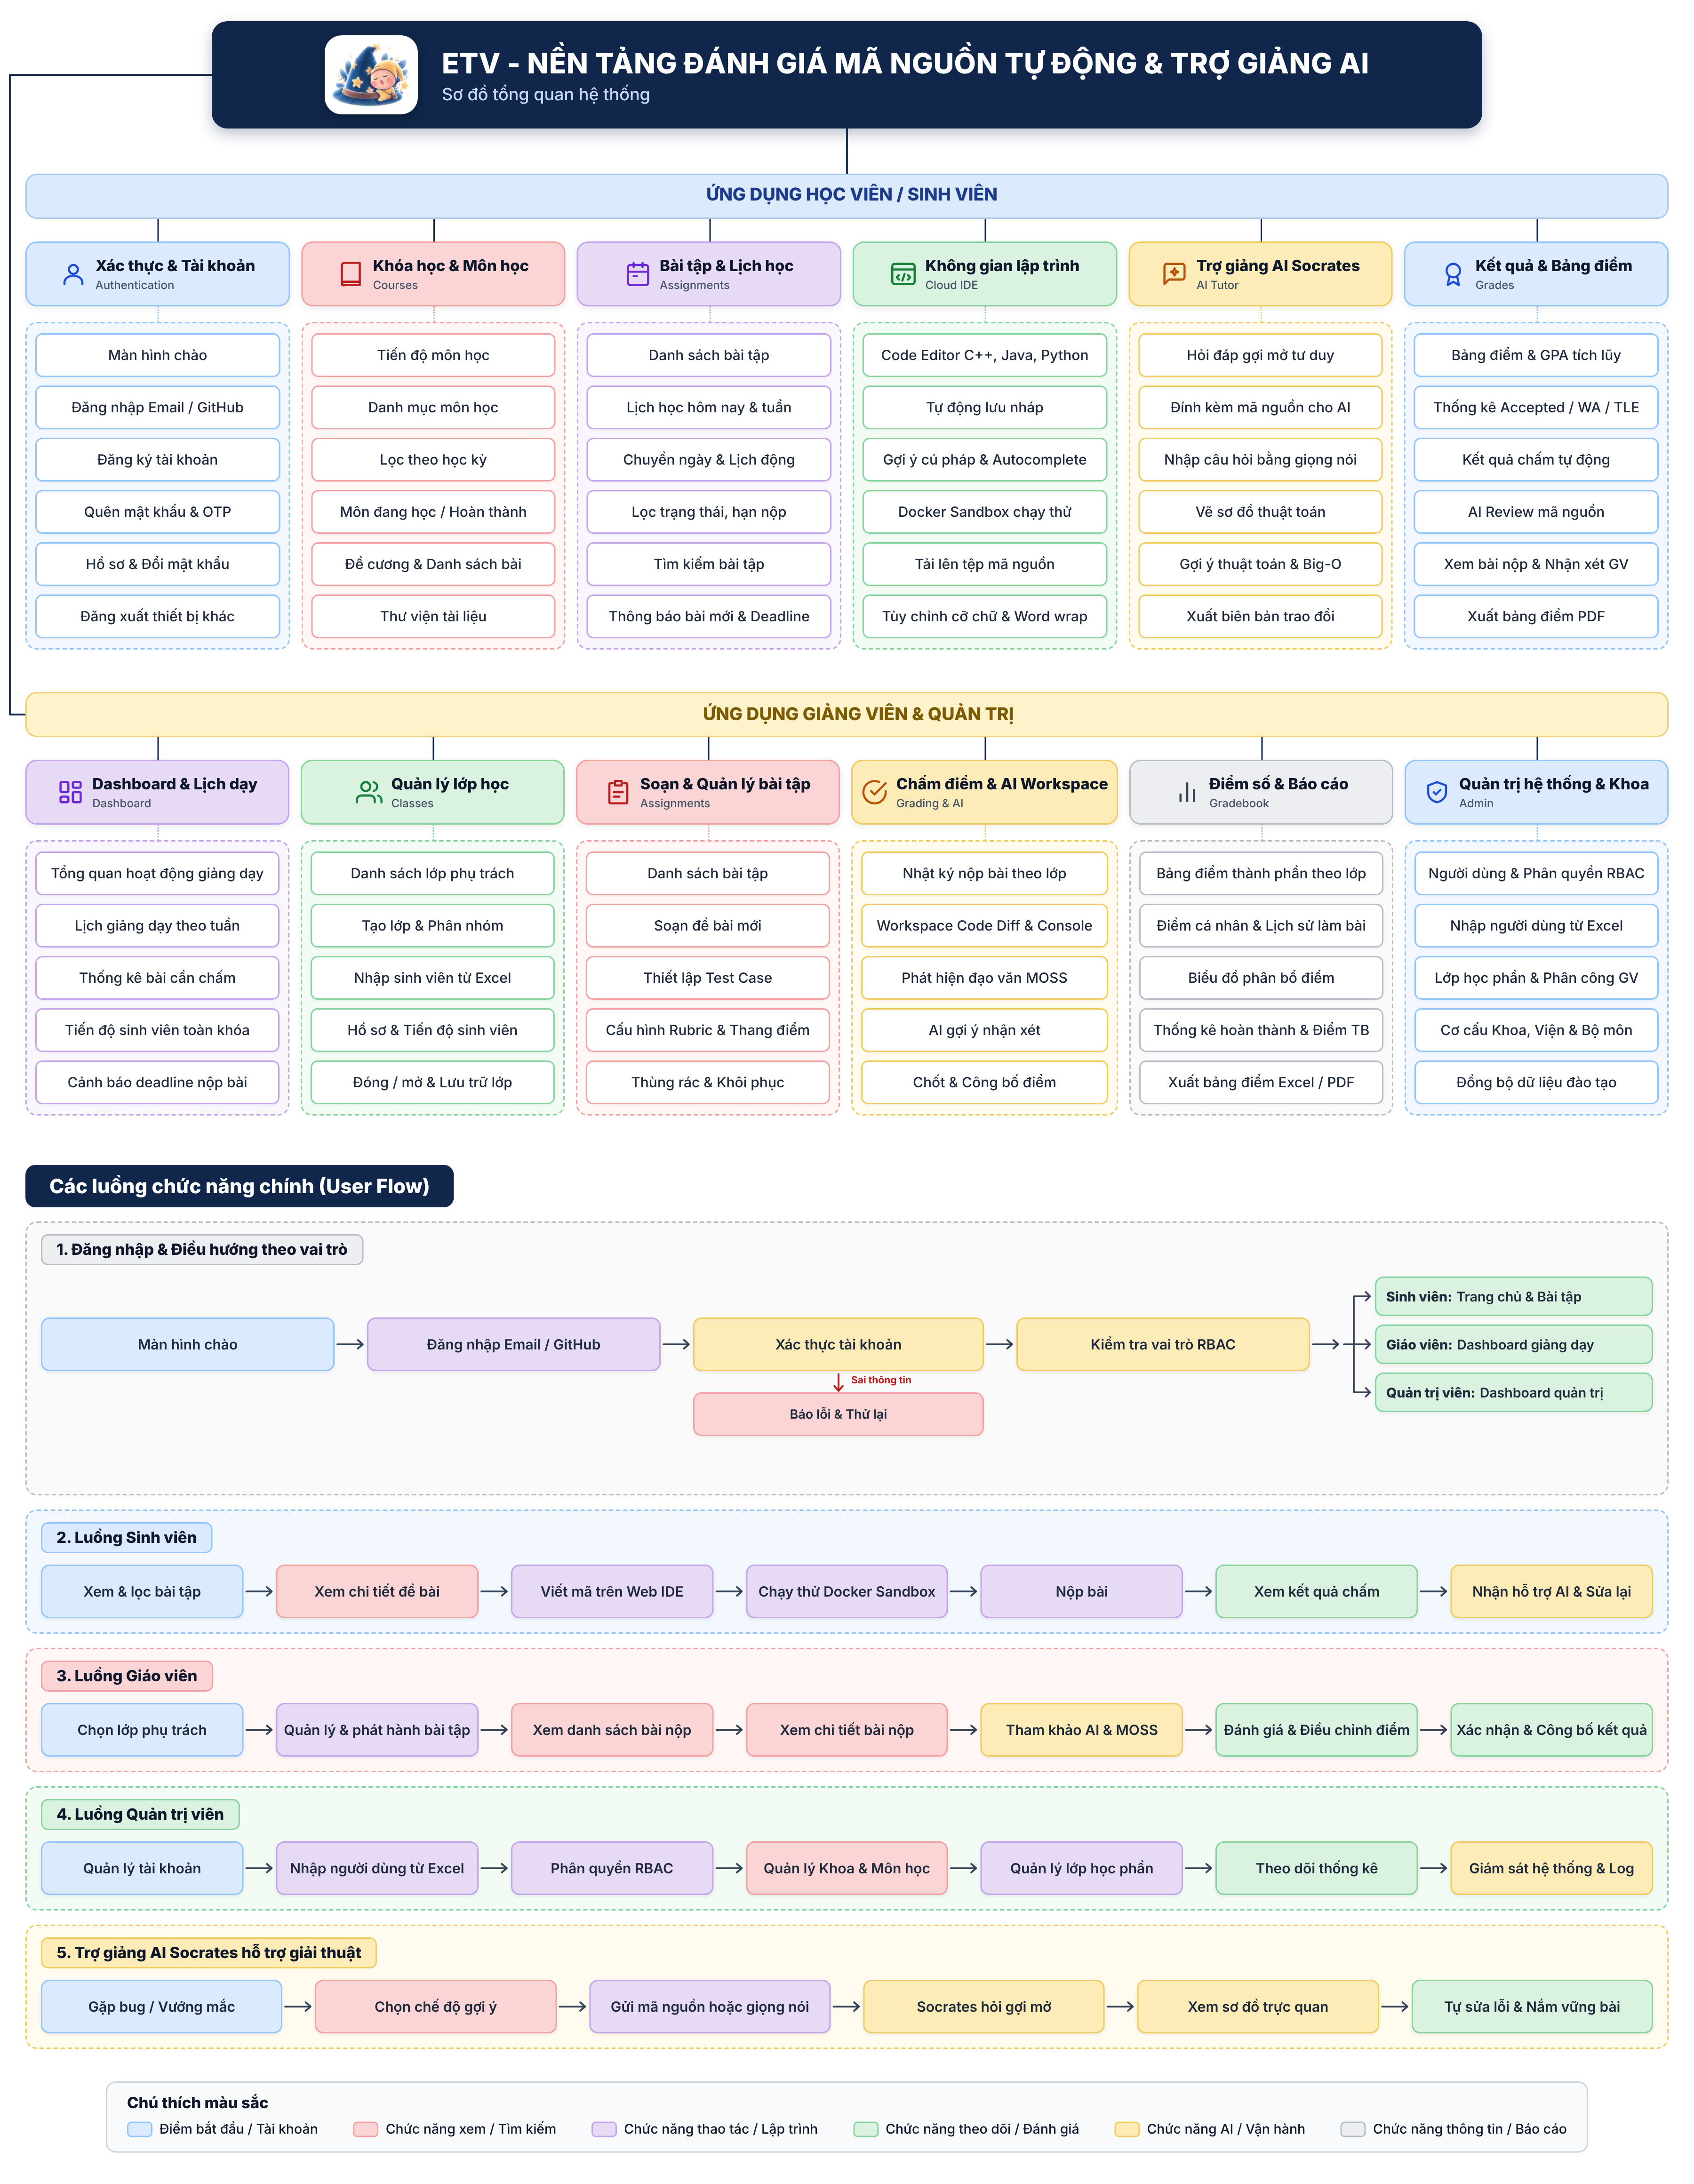
\includegraphics[width=0.88\textwidth]{image2.png}
  \caption{Sơ đồ tổng quan hệ thống và các luồng chức năng chính\label{fig:so_do_tong_quan}}
\end{figure}

\newpage

\section{Xây dựng hệ thống thiết kế}

Nhằm đảm bảo tính nhất quán giữa các phân hệ Giảng viên, Sinh viên và Quản trị viên, nhóm đã xây dựng hệ thống thiết kế đồng bộ cho hệ thống ETV. Hệ thống được tổ chức theo các quy chuẩn về màu sắc, kiểu chữ, thành phần giao diện dùng chung và bố cục đa nền tảng, tạo nền tảng vững chắc cho quá trình lập trình giao diện thực tế \cite{figmaDesignSystem}.

\subsection{Màu sắc, kiểu chữ và quy cách trình bày}

Hệ thống màu sắc trong tệp Figma được phân thành hai tầng: màu gốc (primitive tokens) và màu theo vai trò sử dụng (semantic tokens) nhằm tăng tính trực quan và khả năng mở rộng \cite{figmaDesignSystem}. Quy cách màu sắc chi tiết được trình bày trong Bảng~\ref{tab:mau_sac}.

\begin{table}[htbp]
\centering
\caption{Các màu sắc chính trong hệ thống giao diện ETV\label{tab:mau_sac}}
\begin{tabular}{|p{3.3cm}|p{3.2cm}|p{7.5cm}|}
\hline
\textbf{Vai trò thành phần} & \textbf{Mã màu (HEX)} & \textbf{Quy cách và ngữ cảnh sử dụng thực tế} \\
\hline
Màu bề mặt (surface) & \texttt{\#FEF3C7} \ \colorsample{etvSurface} & Nền vàng kem ấm (Amber) bao phủ toàn bộ các màn hình chức năng. \\
\hline
Màu thanh điều hướng & \texttt{\#1F3B54} \ \colorsample{etvNav} & Nền xanh biển đậm (Deep Teal) của thanh bên Desktop và thanh đáy Mobile. \\
\hline
Mục điều hướng đang chọn & \texttt{\#A1C4E9} \ \colorsample{etvSelected} & Nền xanh pastel dịu làm nổi bật mục trang hiện tại. \\
\hline
Màu chủ đạo (primary) & \texttt{\#0047AB} \ \colorsample{etvPrimary} & Nút và chi tiết cần nhấn mạnh. \\
\hline
Màu chữ chính (ink) & \texttt{\#0F172A} \ \colorsample{etvInk} & Tiêu đề và nội dung quan trọng (tiêu đề trang, tên lớp học, tên môn và các số liệu thống kê lớn). \\
\hline
Màu chữ phụ (muted) & \texttt{\#475569} \ \colorsample{etvMuted} & Tiêu đề và nội dung quan trọng (tiêu đề trang, tên lớp học, tên môn và các số liệu thống kê lớn) \\
\hline
Thành công / cảnh báo / lỗi & \texttt{\#16A34A} \ \colorsample{etvSuccess}\newline \texttt{\#D97706} \ \colorsample{etvWarning}\newline \texttt{\#DC2626} \ \colorsample{etvDanger} & Phân biệt các trạng thái thao tác (xanh lá: đang hoạt động, hoàn thành; vàng cam: cảnh báo hạn nộp; đỏ: đóng lớp, xóa, quá hạn) \\
\hline
\end{tabular}
\end{table}

Về kiểu chữ, giao diện sử dụng phông chữ \textbf{Inter} cho các nội dung văn bản thông thường và \textbf{JetBrains Mono} cho các khối mã nguồn, màn hình Docker Sandbox. Các kiểu chữ được lưu thành Text Style trong Figma: tiêu đề trang chính dùng cỡ 30~px (Bold); tiêu đề mục và phân đoạn dùng cỡ \textbf{20 -- 24~px} (SemiBold); tiêu đề thẻ lớp dùng cỡ \textbf{18~px} (SemiBold); chữ nội dung bảng và mô tả dùng cỡ \textbf{14~px} (Regular); chữ trên nút bấm và nhãn nhập liệu dùng cỡ \textbf{14~px} (Medium/SemiBold); chữ chú thích phụ và thẻ tag dùng cỡ \textbf{12~px} (Regular); các dòng mã lập trình dùng cỡ \textbf{12 -- 14~px} với phông JetBrains Mono để đảm bảo các ký tự thẳng hàng, dễ đọc.

\subsection{Quy chuẩn giao diện và thành phần dùng chung}

Các thành phần giao diện được đóng gói thành các Component và Component Set có khả năng tái sử dụng cao trên Figma \cite{figmaDesignSystem}, bao gồm:
\begin{itemize}
  \item \textbf{Nút bấm (Buttons):} Nút chính (Primary) dùng màu xanh với góc bo \textbf{8 -- 10~px}; nút phụ (Secondary/Outline) dùng viền xám nền trắng; nút nguy hiểm (Danger) dùng màu đỏ cho các thao tác đóng lớp hoặc xóa dữ liệu. Các nút đều được thiết lập đầy đủ các trạng thái tương tác: mặc định, hover, nhấn chuột và vô hiệu hóa \cite{nielsen1994, figmaDesignSystem}.
  \item \textbf{Ô tìm kiếm và bộ lọc:} Ô tìm kiếm cao \textbf{40~px}, bo góc \textbf{8~px}, tích hợp biểu tượng kính lúp và nút xóa nhanh nội dung. Bộ lọc trạng thái được chuẩn hóa thành ba lựa chọn rõ ràng: Tất cả, Đang hoạt động và Đã đóng.
  \item \textbf{Thanh điều hướng (Navigation):} Thanh bên (Sidebar) trên desktop hỗ trợ hai trạng thái: mở rộng \textbf{(260~px)} và thu gọn \textbf{(76~px)}. Thanh điều hướng trên (TopNavbar) cao \textbf{68~px} tích hợp tìm kiếm toàn hệ thống và chuông thông báo. Thanh điều hướng đáy (BottomMobileNav) trên điện thoại cao \textbf{58~px} với vùng chạm tối thiểu \textbf{44 $\times$ 44~px} giúp người dùng dễ dàng thao tác bằng một tay \cite{nielsen1994, wcag22}.
  \item \textbf{Thẻ thông tin và hộp thoại:} Thẻ lớp học bo góc \textbf{12 -- 16~px}, hiển thị đầy đủ mã lớp, tên môn, sĩ số và thanh tiến độ hoàn thành bài tập. Hộp thoại xác nhận (Modal) có góc bo \textbf{16~px}, hiển thị trên lớp nền tối phủ mờ kèm tiêu đề, nội dung cảnh báo và cặp nút Hủy -- Xác nhận.
  \item \textbf{Góc bo và biểu tượng:} Góc bo được phân cấp theo kích thước thành phần: huy hiệu bo \textbf{6 -- 8~px}, ô nhập liệu và nút bấm bo \textbf{8 -- 10~px}, thẻ thông tin và hộp thoại bo \textbf{12 -- 16~px}. Toàn bộ biểu tượng sử dụng bộ vector chuẩn Lucide Icons với kích thước vùng hình \textbf{16 $\times$ 16~px} và \textbf{20 $\times$ 20~px}, luôn gắn liền với nhãn chữ tương ứng.
\end{itemize}

\subsection{Bố cục và thiết kế responsive}

Để đảm bảo giao diện hiển thị đồng bộ, không bị tràn viền hay chồng lấn nội dung, toàn bộ các màn hình được xây dựng dựa trên hệ thống Auto-layout thích ứng theo 4 kích thước khung chuẩn được trình bày tại Bảng~\ref{tab:bo_cuc}.

\begin{table}[htbp]
\centering
\caption{Quy cách bố cục giao diện ETV trên các kích thước màn hình\label{tab:bo_cuc}}
\begin{tabular}{|p{3.3cm}|p{3.2cm}|p{7.5cm}|}
\hline
\textbf{Nền tảng thiết bị} & \textbf{Kích thước khung} & \textbf{Quy cách hiển thị lưới nội dung} \\
\hline
Web Desktop & 1440 $\times$ 960 px & Bố cục danh sách bảng hoặc lưới thẻ rộng, khoảng đệm mép trong 32~px, khoảng cách khối 24~px. \\
\hline
Tablet Landscape (TL) & 1024 $\times$ 768 px & Lưới thẻ 2 cột cân đối, mỗi thẻ rộng 442~px, khoảng cách giữa các thẻ 16~px. \\
\hline
Tablet Portrait (TP) & 768 $\times$ 1024 px & Lưới thẻ 2 cột cân đối, mỗi thẻ rộng 352~px, lề hai bên 24~px, khoảng cách thẻ 16~px. \\
\hline
Mobile (MOB) & 440 $\times$ 956 px & Dồn về 1 cột dọc duy nhất, mỗi thẻ rộng 100\% (408~px), lề hai bên 16~px, khoảng cách thẻ 16~px. \\
\hline
\end{tabular}
\end{table}

Các quy tắc thích ứng bố cục chính bao gồm:
\begin{itemize}
  \item \textbf{Chuyển đổi thanh điều hướng:} Sử dụng thanh bên dọc trên Desktop và Tablet ngang để tận dụng chiều rộng màn hình; chuyển sang thanh điều hướng trên và đáy trên Tablet dọc và Mobile để tối ưu hóa không gian cuộn dọc và vùng thao tác ngón tay \cite{wcag22}.
  \item \textbf{Co giãn thẻ linh hoạt:} Các thẻ dữ liệu tự động thích ứng với chiều rộng hiển thị, từ chế độ nhiều cột trên Desktop chuyển thành 2 cột đều trên Tablet và giãn rộng 100\% (408~px) trên Mobile \cite{wcag22}.
  \item \textbf{Chuyển đổi bảng dữ liệu:} Các bảng danh sách nhiều cột trên Desktop được chuyển đổi thành các thẻ tóm tắt xếp chồng trên Mobile, giúp người dùng theo dõi dữ liệu thuận tiện mà không cần phải cuộn ngang màn hình \cite{wcag22}.
  \item \textbf{Vùng thao tác an toàn:} Các thành phần bấm chạm trên màn hình cảm ứng luôn đảm bảo chiều cao tối thiểu từ 40 -- 48~px và có khoảng cách đệm hợp lý, tránh việc người dùng thao tác nhầm lẫn \cite{wcag22}.
\end{itemize}

Các quy chuẩn và thông số trên phản ánh chính xác cấu trúc của hệ thống giao diện mẫu trên Figma, được liên kết Prototype tương tác đầy đủ, đóng vai trò làm tài liệu tham chiếu kỹ thuật cho giai đoạn phát triển phần mềm tiếp theo.

\newpage

% ==============================================================================
% CHƯƠNG 3
% ==============================================================================
\chapter{ĐÁNH GIÁ KẾT QUẢ VÀ KẾT LUẬN}

\section{Đánh giá kết quả và hạn chế}

Sau quá trình nghiên cứu, phân tích và thiết kế, nhóm đã xây dựng được giao diện UI/UX cho nền tảng Đánh giá Code và Trợ giảng Ảo với các phân hệ chức năng dành cho sinh viên, giảng viên và các nhóm quản trị. Giao diện được thiết kế theo hướng hiện đại, trực quan, có tính nhất quán về màu sắc, bố cục, kiểu chữ và thành phần tương tác. Các luồng chức năng chính như quản lý bài tập, viết và nộp mã nguồn, xem kết quả chấm tự động, trao đổi với trợ giảng ảo và quản lý hoạt động giảng dạy được thể hiện thông qua các màn hình thiết kế và prototype. Bên cạnh đó, nhóm chú trọng khả năng responsive nhằm đảm bảo giao diện thích ứng với máy tính, máy tính bảng và điện thoại di động.

Tuy nhiên, đề tài vẫn còn một số hạn chế. Việc đánh giá trải nghiệm người dùng chủ yếu dựa trên quá trình phân tích yêu cầu và kiểm tra prototype, chưa được kiểm chứng rộng rãi thông qua số lượng lớn người dùng thực tế. Một số tương tác trên prototype mới dừng ở mức mô phỏng, chưa phản ánh đầy đủ hoạt động của hệ thống khi triển khai thực tế. Ngoài ra, việc tối ưu khả năng tiếp cận, hiệu suất hiển thị và trải nghiệm trên nhiều kích thước màn hình vẫn cần được tiếp tục hoàn thiện \cite{nielsen1994, wcag22}.

\section{Kết luận và hướng phát triển}

Đề tài đã đạt được mục tiêu nghiên cứu, phân tích và thiết kế UI/UX cho nền tảng Đánh giá Code và Trợ giảng Ảo. Sản phẩm thiết kế đã thể hiện được các chức năng nghiệp vụ chính, phân chia giao diện theo từng vai trò người dùng và xây dựng các luồng tương tác phù hợp với nhu cầu giảng dạy, học tập và đánh giá lập trình. Thông qua quá trình thực hiện, nhóm đã vận dụng các kiến thức về thiết kế giao diện, trải nghiệm người dùng, kiến trúc thông tin, thiết kế responsive và xây dựng prototype để tạo ra giải pháp giao diện có tính trực quan, đồng bộ và dễ sử dụng.

Trong tương lai, nhóm định hướng tiếp tục hoàn thiện thiết kế dựa trên phản hồi từ người dùng thực tế, thực hiện kiểm thử khả năng sử dụng (Usability Testing) và tối ưu giao diện trên nhiều thiết bị. Đồng thời, nhóm có thể mở rộng các tính năng như cá nhân hóa trải nghiệm học tập, trực quan hóa tiến độ và kết quả học tập, cải thiện giao diện tương tác với trợ giảng AI và bổ sung các công cụ hỗ trợ giảng viên theo dõi, đánh giá sinh viên. Xa hơn, sản phẩm có thể được kết hợp với hệ thống backend và các dịch vụ chấm code tự động để triển khai thành một nền tảng hoàn chỉnh, phục vụ hiệu quả hơn cho hoạt động đào tạo và học tập lập trình \cite{iso9241, nielsen1994, wcag22, combefis2022automated, messer2024automated, kuo2023study}.

\newpage

% ==============================================================================
% TÀI LIỆU THAM KHẢO
% ==============================================================================
\begin{thebibliography}{99}
\addcontentsline{toc}{chapter}{Tài liệu tham khảo}

\bibitem{iso9241}
International Organization for Standardization, \textit{ISO 9241-210:2019 -- Ergonomics of Human-System Interaction -- Part 210: Human-Centred Design for Interactive Systems}. Geneva, Switzerland: ISO, 2019. [Online]. Available: \url{https://www.iso.org/standard/77520.html}

\bibitem{nielsen1994}
J. Nielsen, ``10 Usability Heuristics for User Interface Design,'' Nielsen Norman Group, Apr. 24, 1994. [Online]. Available: \url{https://www.nngroup.com/articles/ten-usability-heuristics/}

\bibitem{wcag22}
World Wide Web Consortium (W3C), ``Web Content Accessibility Guidelines (WCAG) 2.2,'' Dec. 12, 2024. [Online]. Available: \url{https://www.w3.org/TR/WCAG22/}

\bibitem{figmaDesignSystem}
Figma, ``Overview: Introduction to Design Systems,'' Figma Learn. [Online]. Available: \url{https://help.figma.com/hc/en-us/articles/14552901442839-Overview-Introduction-to-design-systems}

\bibitem{combefis2022automated}
S. Combéfis, ``Automated Code Assessment for Education: Review, Classification and Perspectives on Techniques and Tools,'' \textit{Software}, vol. 1, no. 1, pp. 3--30, 2022, doi: 10.3390/software1010002.

\bibitem{messer2024automated}
M. Messer, N. C. C. Brown, M. Kölling, and M. Shi, ``Automated Grading and Feedback Tools for Programming Education: A Systematic Review,'' \textit{ACM Transactions on Computing Education}, vol. 24, no. 1, 2024, doi: 10.1145/3636515.

\bibitem{kuo2023study}
J.-Y. Kuo, Z.-J. Wen, T.-F. Hsieh, and H.-X. Huang, ``A Study on the Security of Online Judge System Applied Sandbox Technology,'' \textit{Electronics}, vol. 12, no. 14, Art. no. 3018, 2023, doi: 10.3390/electronics12143018.

\bibitem{kuo2022study}
J.-Y. Kuo, Z.-J. Wen, H.-X. Huang, and I.-T. Guo, ``The Study on Security Online Judge System Applied Sandbox Technology,'' in \textit{Proc. 2022 IEEE/ACIS 24th Int. Winter Conf. Software Engineering, Artificial Intelligence, Networking and Parallel/Distributed Computing (SNPD)}, Taichung, Taiwan, 2022, pp. 168--172, doi: 10.1109/SNPD54884.2022.10051768.

\end{thebibliography}

\end{document}
